\documentclass[11pt]{article}
\usepackage[margin=1in]{geometry}
\usepackage[T1]{fontenc}
\usepackage[utf8]{inputenc}
\usepackage{lmodern}
\usepackage{microtype}
\usepackage{graphicx}
\usepackage{booktabs}
\usepackage{array}
\usepackage{float}
\usepackage{multirow}
\usepackage{amsmath}
\usepackage{amssymb}
\usepackage{xcolor}
\usepackage{hyperref}
\usepackage{setspace}
\usepackage{enumitem}
\usepackage{longtable}

\hypersetup{
  colorlinks=true,
  linkcolor=blue!50!black,
  filecolor=blue!50!black,
  urlcolor=blue!50!black
}
\setlist[itemize]{topsep=4pt,itemsep=2pt,leftmargin=1.5em}
\setlist[enumerate]{topsep=4pt,itemsep=2pt,leftmargin=1.7em}

\title{From ``Truth Topology'' to Readout Bottlenecks:\\
Negative Replication on GSM8K and a Positive Representation--Decoder Dissociation in Procedural Micro-Worlds}
\author{Marcel \\ Independent Researcher}
\date{April 2026}

\begin{document}
\maketitle
\onehalfspacing

\begin{abstract}
This paper reports a multi-stage study of hidden-state geometry for correctness prediction in language-model reasoning.
The original hypothesis was ambitious: perhaps global topological summaries of hidden-state traces could provide a robust signal of correctness or ``truth.''
That hypothesis did not survive stronger checks.
On GSM8K-style reasoning traces \cite{cobbe2021gsm8k}, dynamic and windowed $H_0$ features were weak, often degenerate, and did not outperform simple controls.
A separate fixed-decoding GSM8K branch yielded a stronger operational result: non-convergence, as measured by token-cap termination, was the dominant predictor of error.

The main positive result emerged only after changing the task.
We introduced a procedural micro-world benchmark with nonce vocabularies, held-out templates, and exact tri-label semantics over \texttt{True}/\texttt{False}/\texttt{Unknown}.
In that setting, a consistent dissociation appeared across Qwen and Gemma families \cite{qwen_model_card,gemma_model_card}: decoder behavior systematically under-expressed \texttt{Unknown}, yet verdict-region hidden-state probes recovered substantial \texttt{Unknown} signal on held-out worlds.
This dissociation survived prompt-path controls, constrained label decoding, base-vs-instruct checks, verdict-step logit analysis, and layer sweeps.
The paper's final claim is therefore narrower and stronger than the original repository framing: semantic non-entailment is internally represented, but often under-realized by decoder readout.
\end{abstract}

\section{Scope and Final Claim}
This project began as a search for a global internal marker of correctness.
The final evidence supports a different claim:
\begin{quote}
In a held-out procedural semantic task, non-entailment (\texttt{Unknown}) is represented in hidden states but systematically under-realized by decoder outputs.
\end{quote}

The paper therefore has three parts:
\begin{enumerate}
  \item a negative replication record for global-topology correctness signals on GSM8K-style traces,
  \item a fixed-decoding convergence analysis showing cap-linked non-convergence as a dominant error mode, and
  \item a positive result on a procedural micro-world benchmark showing a replicated representation--decoder dissociation for non-entailment.
\end{enumerate}

The main contribution is \emph{not} a universal scalar ``topology of truth.''
The stronger result is a readout-bottleneck interpretation supported by multiple controls.

\section{Why the Original Idea Failed}
The original working hypothesis was that correct reasoning might have a cleaner global geometric or topological signature than incorrect reasoning \cite{carlsson2009,bauer2021ripser}.
The basic recipe was:
\begin{enumerate}
  \item run a small model on a reasoning task,
  \item collect token-level hidden states,
  \item treat those hidden states as a point cloud,
  \item compute topological summaries such as connected-component fragmentation ($H_0$) and loop structure ($H_1$), and
  \item ask whether those summaries predict correctness.
\end{enumerate}

The hypothesis was attractive, but the experiments exposed three problems.

\paragraph{Length confounding.}
Prefix-based features changed largely because more points accumulated, not because the underlying reasoning became more truthful.

\paragraph{Degenerate window geometry.}
Fixed-size window preprocessing, especially per-window standardization and whitening, often collapsed windows into nearly geometry-equivalent objects.
This made several windowed $H_0$ summaries almost pure functions of window size.

\paragraph{Task contamination.}
On natural-language math traces, hidden states reflect too many entangled factors at once: reasoning quality, verbosity, formatting drift, stop conditions, and non-convergence.
This makes a single global topology scalar too blunt to isolate correctness.

The failure of the first branch is itself important.
It prevented a misleading positive claim and forced a cleaner task design.

\section{Experimental Trajectory}
\subsection{Phase A: Global Topology on GSM8K (Negative)}
Small paired runs on Qwen3.5-0.8B and Qwen3.5-2B produced weak dynamic-$H_0$ signals on non-capped 2B traces.
Representative pilot numbers were:
\begin{itemize}
  \item \texttt{h0\_entropy\_final AUC = 0.55}
  \item \texttt{peak\_h0\_entropy AUC = 0.55}
  \item \texttt{auc\_h0\_entropy\_per\_token AUC = 0.50}
  \item \texttt{max\_delta\_h0 AUC = 0.60}
\end{itemize}

A corrected fixed-window test did worse:
\begin{itemize}
  \item controls-only AUC: 0.60
  \item corrected-topology-only AUC: 0.20
  \item controls plus corrected-topology AUC: 0.20
\end{itemize}

These numbers are not compatible with a strong correctness-prediction claim.

\subsection{Phase B: Fixed-Decoding GSM8K (Convergence Result)}
A second branch held decoding fixed for Qwen3.5-2B and shifted focus from topology to operational failure mode on a GSM8K slice \cite{cobbe2021gsm8k}.
The key variables were:
\[
C = \mathbf{1}[\text{run terminated by } \texttt{max\_new\_tokens}], \qquad
Y = \mathbf{1}[\text{answer is wrong}].
\]

On a within-question batch of \(n=180\) samples:
\begin{itemize}
  \item capped: 87 samples (75 wrong / 12 correct)
  \item EOS: 93 samples (17 wrong / 76 correct)
  \item AUC(\(C \rightarrow Y\)): 0.839
  \item odds ratio (wrong given cap): 26.40
\end{itemize}

\begin{figure}[H]
  \centering
  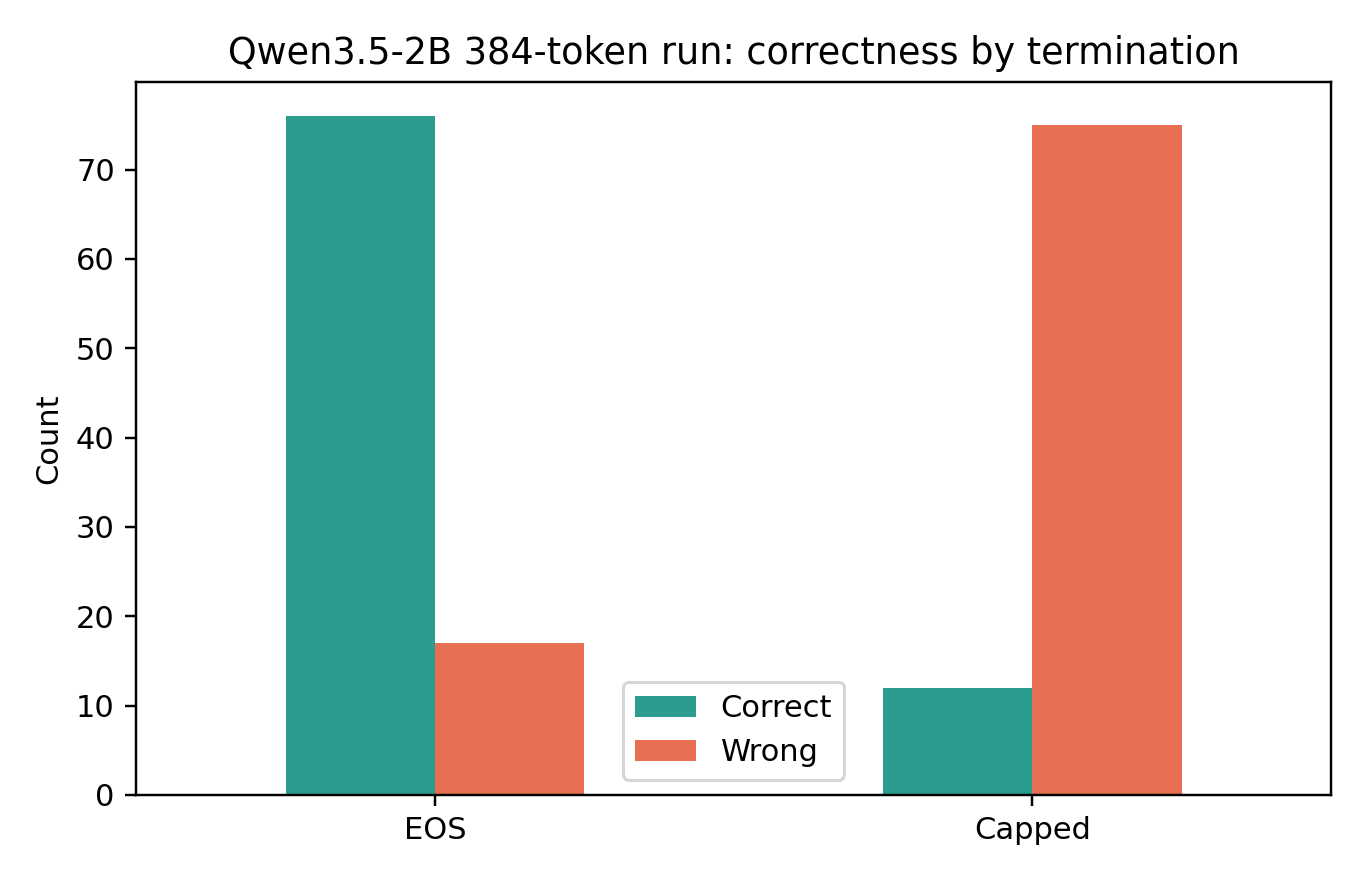
\includegraphics[width=0.72\linewidth]{figures/fig1_convergence_cap_outcomes.png}
  \caption{Fixed-config Qwen3.5-2B run: correctness split by termination mode.}
\end{figure}

The odds ratio calculation is:
\[
\mathrm{OR}
=
\frac{\frac{75}{12}}{\frac{17}{76}}
\approx 26.40.
\]

A matched sensitivity rerun at 640 tokens for the originally capped cases showed that both truncation and deeper non-convergence mattered:
some failures were rescued by a longer budget, but many remained wrong even after receiving more room to continue.

\subsection{Phase C: Procedural Micro-World Semantics (Main Positive Result)}
The project became scientifically cleaner only after replacing benchmark reasoning with a procedurally generated semantic task, in line with controlled-evaluation guidance from recent LM analysis literature \cite{liang2022holistic}.
Each generated world contains:
\begin{itemize}
  \item a latent structured state,
  \item nonce entity names, attribute names, and relation names,
  \item held-out lexicons across train/dev/eval,
  \item held-out paraphrase templates across train/dev/eval,
  \item exact tri-label truth conditions over \texttt{True}, \texttt{False}, and \texttt{Unknown}.
\end{itemize}

Each world yields 72 examples: 9 propositions times 8 paraphrases.
The main sweeps used 20 train worlds and 20 eval worlds.

\section{Task Definition}
Let a world be a finite structured state
\[
w = (E, A, R),
\]
where \(E\) is a set of entities, \(A\) denotes unary predicates (attributes), and \(R\) denotes binary predicates (relations).
A proposition \(\phi\) is rendered into natural language by a paraphrase template.
Its semantic status is one of three classes:
\[
y \in \{\texttt{True},\texttt{False},\texttt{Unknown}\}.
\]
The labels are exact:
\begin{itemize}
  \item \texttt{True}: the world entails \(\phi\),
  \item \texttt{False}: the world entails \(\neg \phi\),
  \item \texttt{Unknown}: neither \(\phi\) nor \(\neg \phi\) is entailed.
\end{itemize}

This matters because \texttt{Unknown} is not a stylistic hesitation label.
It is exact non-entailment under the generator.

\subsection{Worked Micro-World Example}
Table~\ref{tab:world_example} shows one illustrative world/query slice.

\begin{table}[H]
\centering
\caption{Worked micro-world example (illustrative format).}
\label{tab:world_example}
\begin{tabular}{p{0.28\linewidth} p{0.46\linewidth} p{0.14\linewidth}}
\toprule
World fact set & Query statement & Gold label \\
\midrule
\texttt{mep is falm}; \texttt{grel is not falm}; \texttt{nalo foshes sop} &
\texttt{The object mep has property falm.} & True \\
\addlinespace
\texttt{mep is falm}; \texttt{grel is not falm}; \texttt{nalo foshes sop} &
\texttt{The object grel has property falm.} & False \\
\addlinespace
\texttt{mep is falm}; \texttt{grel is not falm}; \texttt{nalo foshes sop} &
\texttt{The relation fosh holds from mep to nalo.} & Unknown \\
\bottomrule
\end{tabular}
\end{table}

\section{What Is Stored for Each Example}
For each example, the pipeline stores:
\begin{itemize}
  \item the rendered prompt,
  \item the gold label,
  \item the emitted label,
  \item correctness and parse status,
  \item token IDs,
  \item selected hidden states,
  \item verdict-step logits for canonical label tokens.
\end{itemize}

The key state locations are:
\begin{itemize}
  \item \texttt{final\_prompt}
  \item \texttt{prompt\_tail\_mean}
  \item \texttt{verdict\_token}
  \item \texttt{verdict\_span\_mean}
\end{itemize}

These are the local decision states of the model near label emission.

\section{Methods}
\subsection{Linear Probe}
Take a hidden state from one example at one chosen location:
\[
h \in \mathbb{R}^d.
\]
Each example provides a pair \((h_i, y_i)\), where \(y_i \in \{1,2,3\}\) corresponds to \texttt{True}, \texttt{False}, or \texttt{Unknown}.

A linear probe is
\[
W \in \mathbb{R}^{3\times d}, \qquad b \in \mathbb{R}^3
\]
with class scores
\[
s = Wh + b
\]
and prediction
\[
\hat y = \arg\max_c s_c.
\]
Training minimizes multiclass cross-entropy:
\[
\mathcal{L}(W,b) = -\sum_i
\log \frac{\exp((Wh_i+b)_{y_i})}{\sum_c \exp((Wh_i+b)_c)}.
\]

This probe is intentionally weak and follows the standard linear-probe setup \cite{alain2016probes}.
If it succeeds, the information is already arranged in hidden space in a directly readable linear form.

\subsection{Within-World Geometry Gap}
For one world and one state key, with distance \(d(\cdot,\cdot)\):
\[
D_{\text{same}} = \mathbb{E}[d(h_i,h_j) \mid y_i = y_j],
\]
\[
D_{\text{diff}} = \mathbb{E}[d(h_i,h_j) \mid y_i \neq y_j].
\]
Define the world-level gap:
\[
\Delta = D_{\text{diff}} - D_{\text{same}}.
\]
A positive \(\Delta\) means same-label states are more tightly organized than different-label states.

\subsection{Verdict-Step Label-Logit Metrics}
Let verdict-step logits for canonical label tokens be
\[
\ell_T,\ \ell_F,\ \ell_U.
\]
Then
\[
p(c \mid h) = \frac{e^{\ell_c}}{e^{\ell_T}+e^{\ell_F}+e^{\ell_U}},
\]
with the Unknown competitiveness margin
\[
m_U = \ell_U - \max(\ell_T,\ell_F).
\]
If \(m_U < 0\), Unknown is under-ranked against the strongest non-Unknown candidate.

\subsection{Layer Sweeps}
For each layer \(\ell\), evaluate the same probe protocol and report
\[
R_U^{(\ell)} = \text{Unknown recall of the probe at layer }\ell.
\]
This reveals where non-entailment is maximally linearly recoverable in the network.

\section{Main Micro-World Results}
\subsection{Decoder Behavior vs Hidden-State Recoverability}
Table~\ref{tab:decoderprobe} summarizes the central result on held-out eval worlds.

\begin{table}[H]
\centering
\caption{Decoder behavior vs verdict-token probe on held-out eval worlds (\(n=1440\) examples per model).}
\label{tab:decoderprobe}
\begin{tabular}{lccc}
\toprule
Model & Decoder accuracy & Decoder Unknown recall & Probe Unknown recall \\
\midrule
Qwen3.5-2B & 0.436 & 0.000 & 0.738 \\
Qwen3.5-4B (no-think) & 0.478 & 0.000 & 0.129 \\
Gemma-3-4B-it (no-think) & 0.397 & 0.013 & 0.563 \\
\bottomrule
\end{tabular}
\end{table}

\begin{figure}[H]
  \centering
  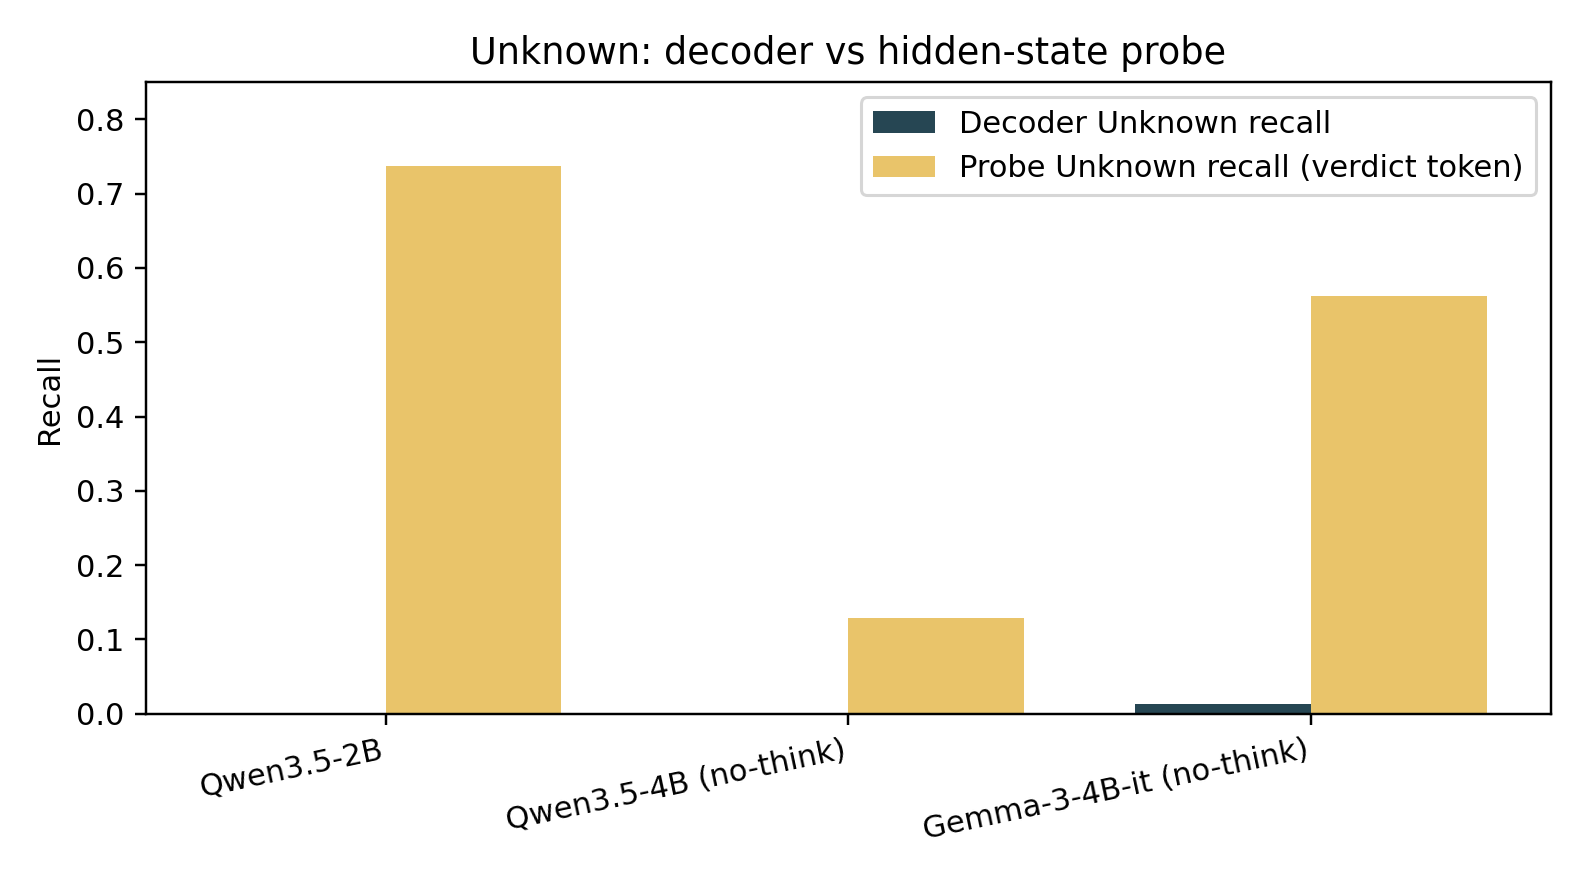
\includegraphics[width=0.80\linewidth]{figures/fig2_unknown_decoder_vs_probe.png}
  \caption{Unknown recall: decoder outputs vs verdict-token probe.}
\end{figure}

The key pattern is not raw accuracy.
It is the gap between emitted-\texttt{Unknown} behavior and hidden-state recoverability of \texttt{Unknown}.

\subsection{World-Level Geometry Consistency}
World-level same-vs-different label distance gaps were positive in every evaluated world for main state keys in both Qwen3.5-2B and Gemma-3-4B-it.

\begin{figure}[H]
  \centering
  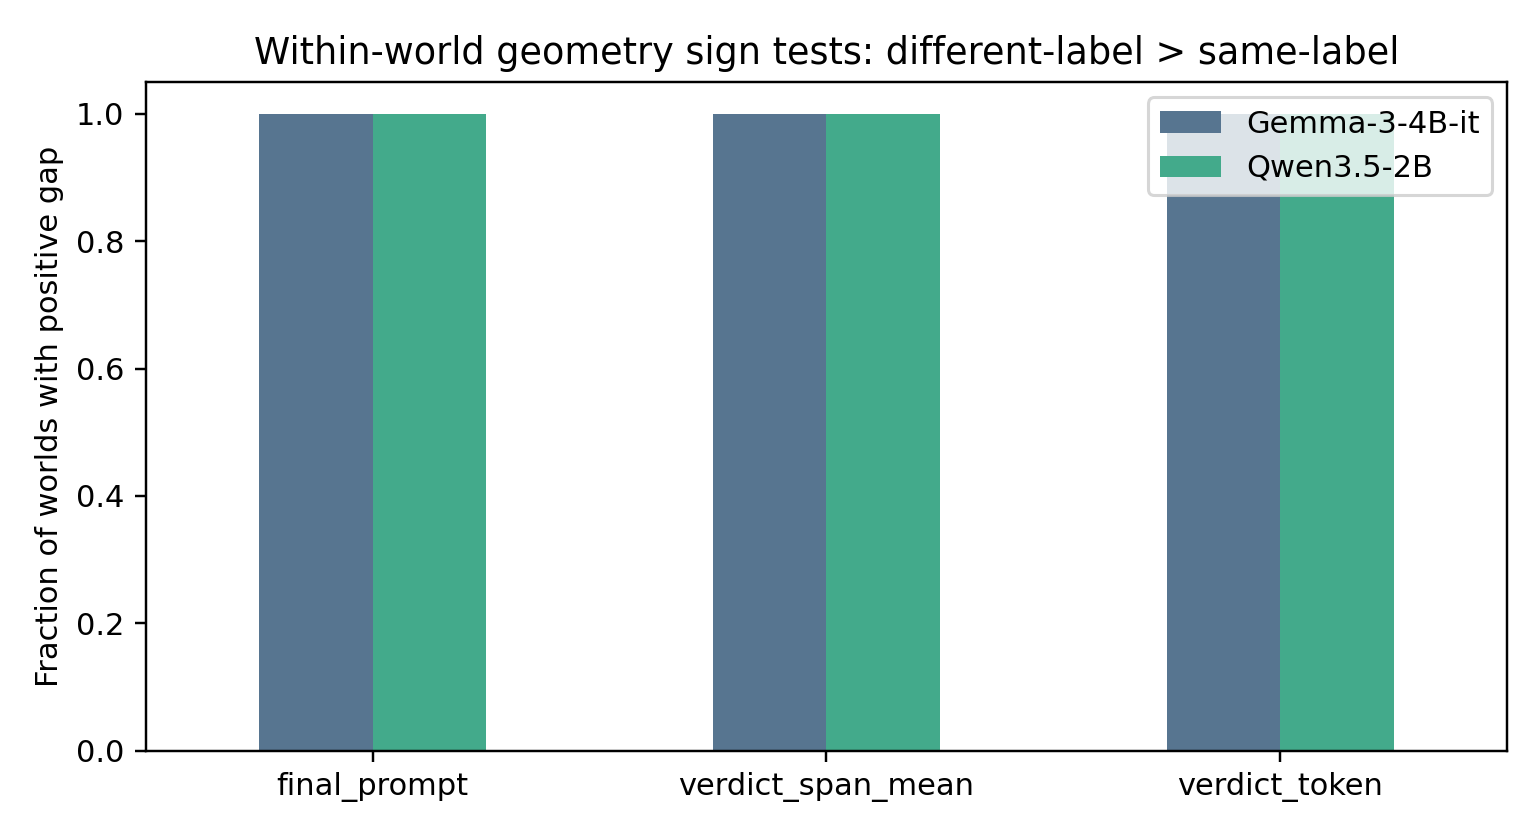
\includegraphics[width=0.72\linewidth]{figures/fig5_geometry_sign_tests.png}
  \caption{Fraction of worlds with positive same-vs-different label distance gap.}
\end{figure}

\subsection{Cross-Family Replication}
The dissociation replicates across Qwen and Gemma:
\begin{enumerate}
  \item decoder outputs under-express \texttt{Unknown},
  \item hidden states still encode \texttt{Unknown},
  \item the gap survives held-out worlds, held-out lexicons, and held-out templates.
\end{enumerate}

\section{Mechanistic Controls}
\subsection{Constrained Decoding}
To test whether free-form decoding alone caused the issue, decoding was constrained to \{\texttt{True}, \texttt{False}, \texttt{Unknown}\}.
This did not repair Unknown collapse in the main models.

\subsection{Prompt-Path Control}
Raw-prompt controls were used to rule out chat-template-only explanations.
The core dissociation remained.

\subsection{Base vs Instruct}
Gemma base initially showed severe parse failures under an unsuitable prompt path.
After repairing prompt format with a base-specific label format, the parse confound disappeared.
Yet base still showed decoder Unknown collapse while probes recovered substantial Unknown signal.

\section{Verdict-Step Label-Logit Analysis}
For gold-\texttt{Unknown} decoder failures:
\begin{itemize}
  \item Gemma-3-4B-it: mean \(P(\texttt{Unknown})=0.192\), mean margin \(m_U=-1.293\),
  \item Gemma-3-4B-pt (basefmt): mean \(P(\texttt{Unknown})=0.177\), mean margin \(m_U=-1.045\).
\end{itemize}
So Unknown is often present but not competitive enough at final label-token competition.

\begin{figure}[H]
  \centering
  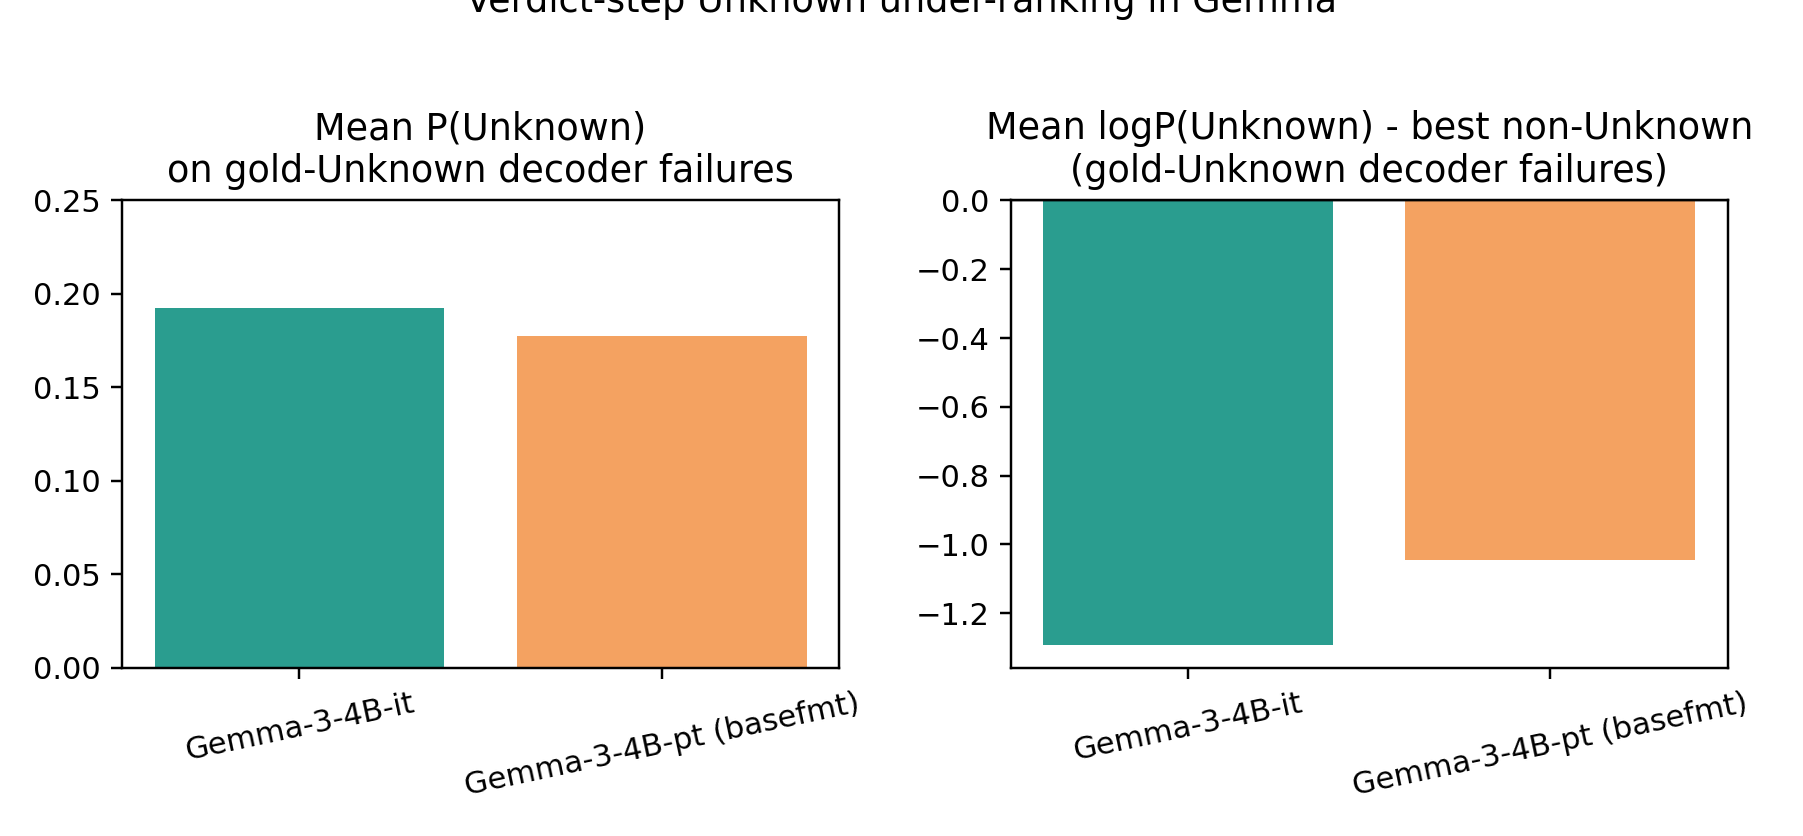
\includegraphics[width=0.86\linewidth]{figures/fig3_gemma_unknown_logit_competitiveness.png}
  \caption{Unknown under-ranking at verdict step on gold-Unknown decoder failures.}
\end{figure}

\section{Layer Sweeps}
The best Unknown recall by state family was:
\begin{itemize}
  \item Gemma-3-4B-it: \texttt{prompt\_last} 0.779 at layer 1, \texttt{verdict\_token} 0.742 at layer 10
  \item Gemma-3-4B-pt (basefmt): \texttt{prompt\_last} 0.825 at layer 29, \texttt{verdict\_token} 0.733 at layer 28
\end{itemize}
This shows strong recoverable Unknown signal exists internally in both instruct and base variants, even when emitted behavior still collapses that class.

\begin{figure}[H]
  \centering
  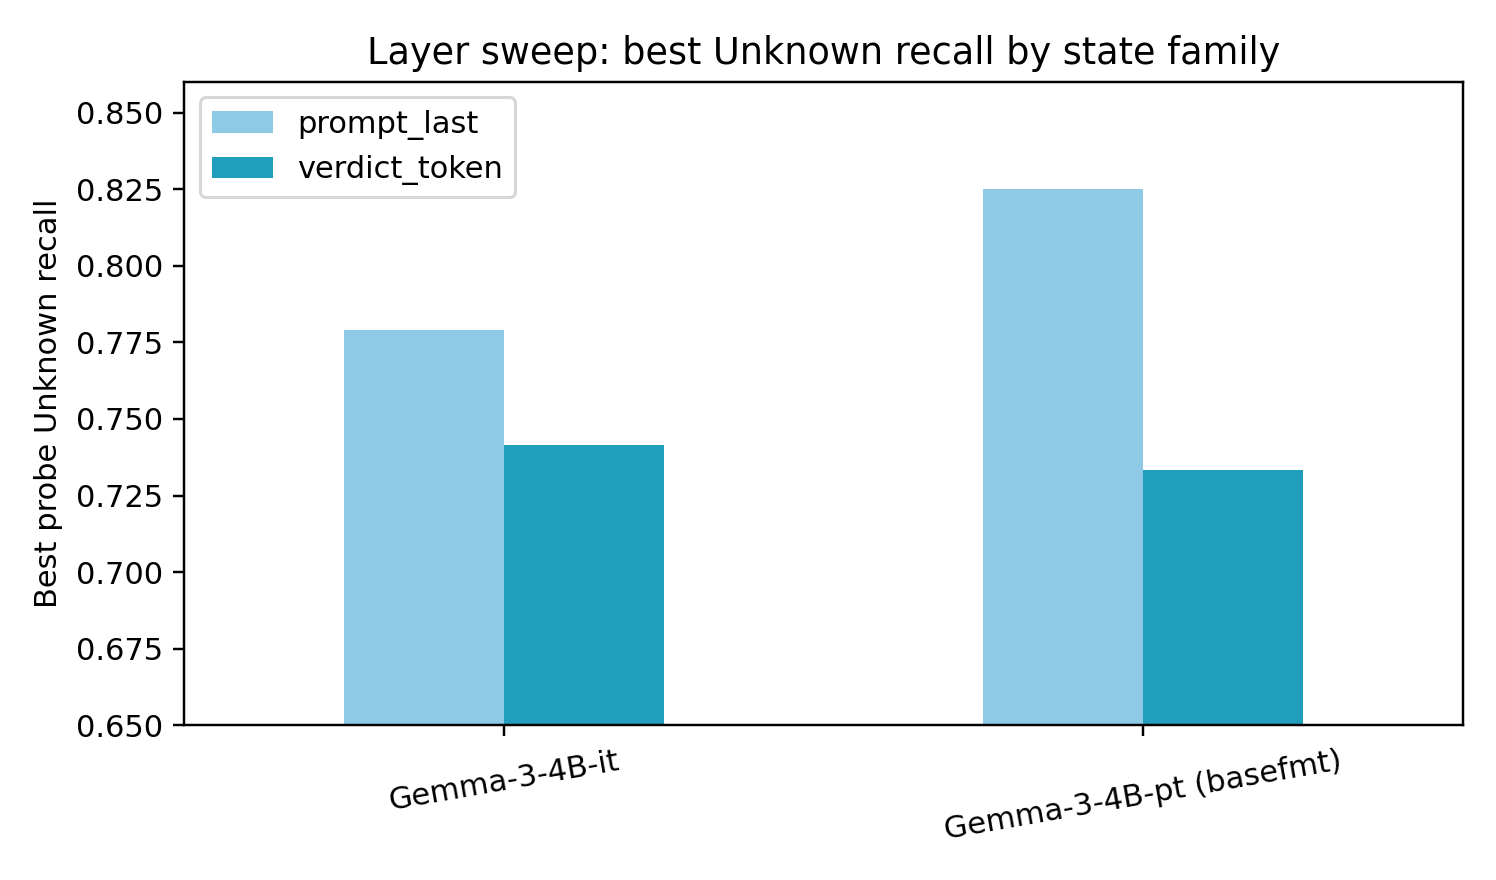
\includegraphics[width=0.76\linewidth]{figures/fig4_layer_sweep_unknown_recall.png}
  \caption{Best Unknown recall from layer sweeps by state family.}
\end{figure}

\section{Interpretation}
The combined evidence supports a readout-bottleneck interpretation:
\begin{enumerate}
  \item semantic non-entailment is encoded internally,
  \item decoder outputs under-express that class,
  \item the mismatch is replicated across model families and controls,
  \item verdict-step logits under-rank Unknown,
  \item layer sweeps show strong internal signal upstream of failed readout.
\end{enumerate}

This is stronger and narrower than the original repository framing.
Results do \emph{not} support a universal ``truth topology'' scalar.

\section{Why This Should Survive Review}
The result survives the obvious reviewer attacks:
\begin{itemize}
  \item \textbf{Memorization objection}: nonce vocabularies, held-out lexicons, held-out templates.
  \item \textbf{Single-family objection}: replicated in both Qwen and Gemma.
  \item \textbf{Template objection}: raw-prompt controls.
  \item \textbf{Parse objection}: Gemma base rerun with repaired prompt format.
  \item \textbf{Free-decoding objection}: constrained decoding tested.
  \item \textbf{``No internal Unknown'' objection}: probes, geometry, logits, and layer sweeps all counter it.
\end{itemize}

No single analysis carries the paper; strength comes from triangulation.

\section{Practical Artifact Map}
Key outputs used in the paper:
\begin{itemize}
  \item convergence branch: \texttt{artifacts/qwen35\_2b\_within\_question/analysis/}
  \item cap sensitivity: \texttt{artifacts/qwen35\_2b\_cap\_sensitivity\_640/analysis/}
  \item cross-model decoder comparisons: \texttt{artifacts/micro\_world\_v1/comparison\_decoder\_*.csv}
  \item probe comparisons: \texttt{artifacts/micro\_world\_v1/comparison\_probe\_states\_*.csv}
  \item constrained-decoding comparisons: \texttt{artifacts/micro\_world\_v1/comparison\_decoder\_constrained\_*.csv}
  \item verdict-step logits: \texttt{artifacts/micro\_world\_v1/label\_logits\_*/}
  \item layer sweeps: \texttt{artifacts/micro\_world\_v1/layer\_sweep\_*/}
\end{itemize}

\section{Limitations}
\begin{itemize}
  \item The micro-world benchmark is synthetic, even though controlled and compositional.
  \item Model coverage is small-to-mid scale; larger-scale behavior is open.
  \item Probe recoverability does not prove causal use by decoder policy.
  \item The exact source of readout failure is not fully decomposed; it may involve calibration, label competition, or post-training behavior shaping.
\end{itemize}

\section{Reproducibility}
Locked dependency snapshot:
\texttt{repro/requirements.lock.txt}

Figure generation:
\begin{verbatim}
python3 paper/scripts/make_figures.py
\end{verbatim}

Compile:
\begin{verbatim}
cd paper
pdflatex -interaction=nonstopmode -halt-on-error main.tex
pdflatex -interaction=nonstopmode -halt-on-error main.tex
\end{verbatim}

\section{Conclusion}
The original ``truth topology'' objective was too broad for the observed evidence.
The final validated contribution is a replicated representation--decoder dissociation:
semantic non-entailment is strongly encoded in hidden states but systematically under-surfaced at output time.
The correct framing is no longer a search for a single topology-of-truth scalar, but a study of how semantic uncertainty is preserved internally and lost at decoder readout.

\section*{References}
\begin{thebibliography}{99}

\bibitem{alain2016probes}
Guillaume Alain and Yoshua Bengio.
\newblock Understanding intermediate layers using linear classifier probes.
\newblock In \emph{ICLR Workshop Track}, 2016.

\bibitem{bauer2021ripser}
Ulrich Bauer.
\newblock Ripser: efficient computation of Vietoris--Rips persistence barcodes.
\newblock \emph{Journal of Applied and Computational Topology}, 5:391--423, 2021.

\bibitem{carlsson2009}
Gunnar Carlsson.
\newblock Topology and data.
\newblock \emph{Bulletin of the American Mathematical Society}, 46(2):255--308, 2009.

\bibitem{cobbe2021gsm8k}
Karl Cobbe, Vineet Kosaraju, Mohammad Bavarian, Mark Chen, Heewoo Jun, Lukasz Kaiser, Matthias Plappert, Jerry Tworek, Jacob Hilton, Reiichiro Nakano, Christopher Hesse, and John Schulman.
\newblock Training verifiers to solve math word problems.
\newblock arXiv:2110.14168, 2021.

\bibitem{gemma_model_card}
Google.
\newblock Gemma 3 4B Instruct model card.
\newblock \url{https://huggingface.co/google/gemma-3-4b-it}. Accessed 2026-04-14.

\bibitem{liang2022holistic}
Percy Liang, Rishi Bommasani, Tony Lee, et al.
\newblock Holistic evaluation of language models.
\newblock \emph{Transactions on Machine Learning Research}, 2023.

\bibitem{qwen_model_card}
Qwen Team.
\newblock Qwen3.5 model family card.
\newblock \url{https://huggingface.co/Qwen/Qwen3.5-4B}. Accessed 2026-04-14.

\end{thebibliography}

\appendix
\section{Appendix A: Full Reproduction Commands}
\begin{verbatim}
# Phase A dynamic topology
python3 scripts/analyze_paired_dynamic.py \
  --artifact-08b artifacts/paired_qwen35_08b_10 \
  --artifact-2b artifacts/paired_qwen35_2b_10 \
  --out-dir artifacts/paired_dynamic_qwen35

# Phase A corrected window test
python3 scripts/analyze_2b_window_corrected.py \
  --artifact-dir artifacts/paired_qwen35_2b_10 \
  --out-dir artifacts/qwen35_2b_window_corrected

# Phase B fixed-decoding run
python3 scripts/run_multi_sample_questions.py \
  --model-id Qwen/Qwen3.5-2B \
  --question-start 0 --question-count 20 --samples-per-question 9 \
  --temperature 0.7 --top-p 0.95 --max-new-tokens 384 \
  --artifact-dir artifacts/qwen35_2b_within_question

# Phase B cap sensitivity
python3 scripts/run_cap_sensitivity.py \
  --model-id Qwen/Qwen3.5-2B \
  --source-artifact-dir artifacts/qwen35_2b_within_question \
  --out-dir artifacts/qwen35_2b_cap_sensitivity_640 \
  --temperature 0.7 --top-p 0.95 --max-new-tokens 640

# Phase C dataset
python3 scripts/generate_micro_world_dataset.py \
  --out-dir artifacts/micro_world_v1/dataset \
  --seed 1729 --train-worlds 100 --dev-worlds 25 --eval-worlds 100 \
  --props-per-world 9 --paraphrases-per-prop 8
\end{verbatim}

\end{document}
